\section{Experimentation}
\label{sec:experimentation}

In this section, we evaluate the benefits that \SPRAY can bring to
protocols built on top of it. Using the example of a broadcast
mechanism, we expect \SPRAY to keep a stable delivery rate on messages
while supporting network size variations. Then, we evaluate how the
adaptiveness of \SPRAY impacts common metrics of peer sampling
performance including clustering coefficient, average shortest path
length, in-degree distribution, robustness, and arc count. We compare \SPRAY with
a representative of fixed-size partial view approaches, namely
\CYCLON. We expect \SPRAY and \CYCLON to exhibit similar behaviors
when \CYCLON is optimally configured in advance to handle the network
size. We expect \SPRAY to save resources when \CYCLON is oversized,
and to be more robust when \CYCLON is undersized. Finally, we expect
\SPRAY to keep a negligible number of duplicates in its partial
views. We also evaluate the impact of the WebRTC connection establishment
on \CYCLON, \SCAMP, and \SPRAY, in  networks subject to message loss.
We expect a normal behavior for \CYCLON and \SPRAY while \SCAMP becomes
quickly partitioned.
The experiments run on the \PEERSIM
simulator~\cite{montresor2009peersim}. The code of the random peer
sampling protocols is available on the Github
platform\footnote{\url{https://github.com/justayak/peersim-spray}}.

% We use \SCAMP as a baseline for experiments relative to
% connection failures. Unlike \SCAMP, we expect \SPRAY to
% tolerate connection failures.


%%Figure~\ref{fig:architecture} depicts

% The right part of the figure corresponds to the catch up strategy where a member
% may have missed operations due to dropped messages, or simply because the user
% worked on offline mode for a while. Therefore, it regularly asks to its
% neighborhood the missing operations using the differences of version vectors.

%%Using such decentralized collaborative editor, we created real-time editing
%%session on the Grid'5000 testbed involving uptill 600 browsers.


%%\subsection{Spray's properties}

%%The rest of this experimentation section aims to highlight different properties
%%of \SPRAY through large scale simulations.

%\vspace{-7pt}
%%\paragraph{Clustering and convergence time}

\subsection{Delivery rate on broadcast}

\begin{figure}
  \begin{center}
    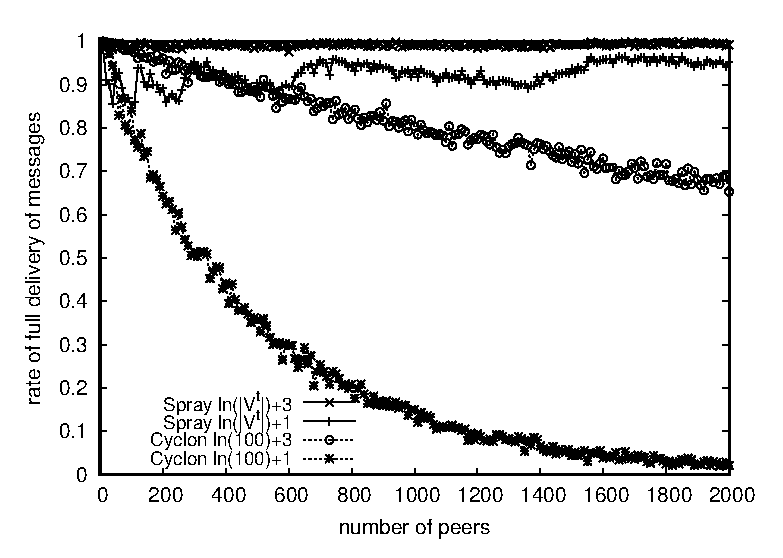
\includegraphics[width=0.49\textwidth]{img/hardrate.eps}
    \caption{\label{fig:hardrate}Ratio of messages delivered to all peers.}
  \end{center}
\end{figure}

\begin{asparadesc}
\item [Objective:] To show how broadcast protocols can benefit from
  an adaptive random peer sampling protocol.
\item [Description:] Broadcast protocols extensively use the partial
  views provided by random peer sampling protocols to efficiently
  disseminate messages to all the network. A broadcasting peer chooses
  some neighbors from its partial view to whom it sends the
  message. Each peer receiving such a message broadcasts it once, in
  an identical way. The message transitively reaches all members. The
  number of chosen neighbors is called the \emph{fanout}. Since
  several applications need to broadcast messages more frequently than
  they can shuffle their neighbors, broadcast protocols tend to use
  view sizes that are much larger than the broadcast
  fanout~\cite{Frey09Middleware}. This allows the peer-sampling
  protocol to provide the application with fresh peers at each
  broadcast round without having to wait for the network's mixing
  time~\cite{jelasity2007gossip}. In this experiment, we consider an
  application configured to target approximately $100$ peers: a user
  streaming the live video of a local sport event. We configure
  \CYCLON's partial view to $6$ times the threshold fanout required
  for $100$ nodes ($6 \ln(100) \approx 6 \cdot 5 = 30$), and consider
  two configurations for the broadcast fanout $\ln(100)+1 \approx 6 $
  and $\ln(100)+3 \approx 8$, which provide high reliability with
  $100$ nodes. Similarly, we configure \SPRAY to have partial views
  size equal to $6 \cdot \ln(|V^t|)$---instead of adding only 1 arc
  targeting its contact (cf. Section \ref{subsec:joining}), the
  newcomer adds 6 arcs---and set the fanout to one sixth of the view
  size plus $1$ or $3$. This gives both protocols the same
  configuration for $100$ nodes.  We then consider network sizes
  varying between $100$ and $2000$ peers, and measure the full
  delivery rate of 1k messages, i.e., we evaluate the fraction of
  messages that reach all the members of the network.
\item [Results:] Figure~\ref{fig:hardrate} shows the result of this
  experiment. First, we observe that the rate of messages delivery
  using \CYCLON suffers from a steady decrease. The highest fanout
  leads to better results. In contrast, \SPRAY remains stable despite
  the presence of small jumps. A fanout set to $\ln(|V^t|)+1$ gives a
  full delivery rate above 90\%. A fanout set to $\ln(|V^t|)+3$ is
  very close to 100\%. Overall, the broadcast mechanism benefits from
  the adaptive nature of \SPRAY's partial view, which allows it to
  scale according to the size of the network.
\item [Reasons:] From~\cite{erdos1959random}, we know that the sharp
  threshold of connectedness of random graphs is
  $\Theta(\ln(|V|))$. Regarding the broadcast, this means that, with a
  sufficiently random and large partial view, a fanout set accordingly
  provides a full delivery rate of about 50\%. At this point,
  increasing the fanout improves drastically the resulting rate, but
  the contribution of each increment diminishes with respect to the
  previous increment. The broadcast protocol built on top of \CYCLON
  has a constant fanout set for a specific network size. As long as
  the network is smaller than this value, the full delivery rate stays
  high. However, it quickly decreases with larger network sizes.
  \SPRAY instead allows the application fanout to follow the growth of
  the partial view size, which scales logarithmically compared to the
  network size. This allows the application to adapt to changes in the
  size of the network. As a result, the full delivery rate provided by
  the broadcast mechanism on top of \SPRAY remains stable. Since the
  values manipulated by peers---partial view size and fanout---are
  integers, the measurements make small jumps when a rounded value
  increases enough to be incremented.
\end{asparadesc}

% \begin{figure}
%   \begin{center}
%     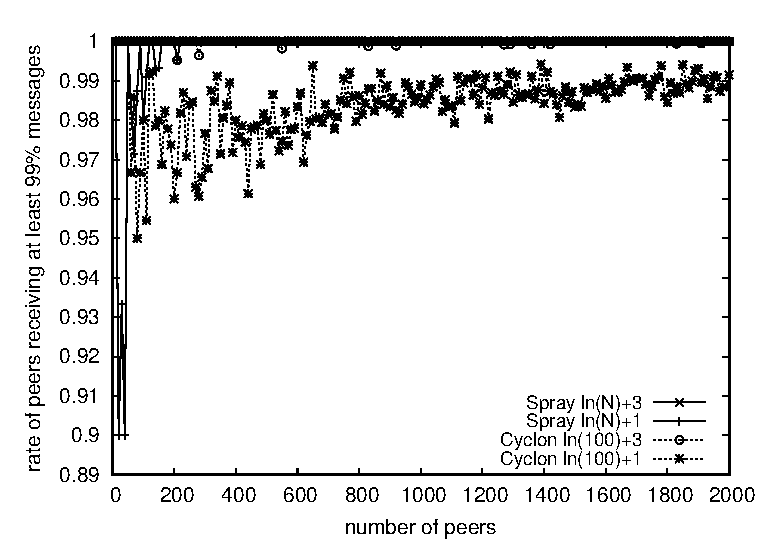
\includegraphics[width=0.49\textwidth]{img/ninetynine.eps}
%     \caption{\label{fig:ninetynine}Ratio of peers which received 99 percent of
%       messages.}
%   \end{center}
% \end{figure}

% \begin{figure}
%   \begin{center}
%     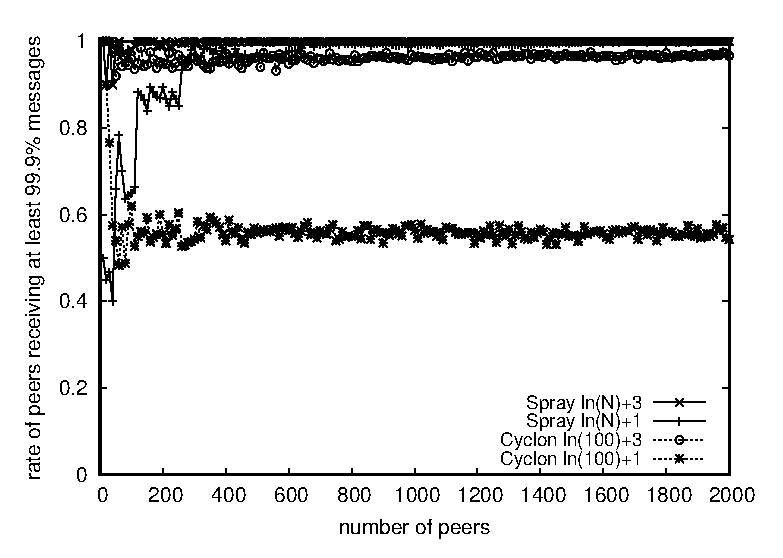
\includegraphics[width=0.49\textwidth]{img/ninetyninedotnine.eps}
%     \caption{\label{fig:ninetyninedotnine}Ratio of peers which received 99.9 percent of
%       messages.}
%   \end{center}
% \end{figure}


\begin{figure}
  \begin{center}
    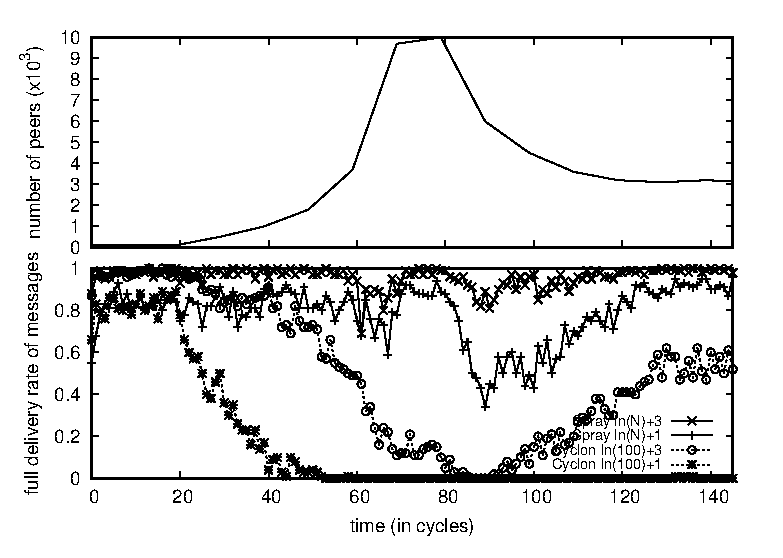
\includegraphics[width=0.49\textwidth]{img/peak.eps}
    \caption{\label{fig:peak}Full delivery rate of messages during a buzz.}
  \end{center}
\end{figure}

\ \\

\begin{asparadesc}
\item [Objective:] To show how the full delivery rate behaves during a buzz,
  i.e., a sudden massive increasing of network size shortly followed by
  departures.
\item [Description:] We configure \SPRAY and \CYCLON like in the
  previous experiment. For \CYCLON, we use a partial view size of 30
  and two broadcast fanout values: $\ln(100)+1$ and $\ln(100)+3$. For
  \SPRAY, we use a dynamic view of $6 \cdot \ln(|V^t|)$ and broadcast
  fanout values of $\ln(|V^t|)+1$ and $\ln(|V^t|)+3$. The simulation
  starts with 100 peers. The network quickly reaches 10k peers during
  the popularity burst. Then the network size decreases to 3k
  members. In this experiment, we measure the full delivery rate over
  each group of 100 consecutive messages.
\item [Results:] Figure~\ref{fig:peak} shows the results of this
  experiment. The top part of the figure shows the evolution of the
  network size over time. The bottom figure shows the full delivery
  rate over time. Like in the previous experiment,
  Figure~\ref{fig:peak} shows that using \CYCLON and a predefined
  fanout works well until the network size reaches an unexpected
  size. During the peak, the delivery rate falls quickly. Conversely,
  the broadcast mechanism built on top of \SPRAY automatically adapts
  the fanout to the size of the network. Thus, it does not experience
  performance losses while a large number of nodes suddenly join, even
  though we observe a decrease in delivery rate during the departures
  of peers, in particular with a fanout of $\ln(|V|)+1$. Overall, the
  broadcast mechanisms involving \SPRAY are more resilient to quick
  membership changes.
\item [Reasons:] The fanout of configurations involving \CYCLON is
  constant. When the number of peers in the network exceeds the
  expectations, the delivery rate quickly degenerates. Concerning
  \SPRAY, the fanout follows the evolution of the network thanks to
  adaptive partial views. Both \SPRAY, and \CYCLON detect departing
  nodes during the shuffling phase. The associated delay leads to the
  use of some stale arcs from partial views, which explains the
  temporary decrease in delivery rate during the shrinking
  phase. Since both \CYCLON and \SPRAY clean their partial views over
  time, the delivery rate recovers its expected value.
\end{asparadesc}

\subsection{Clustering and convergence time}

\begin{figure}
  \centering
  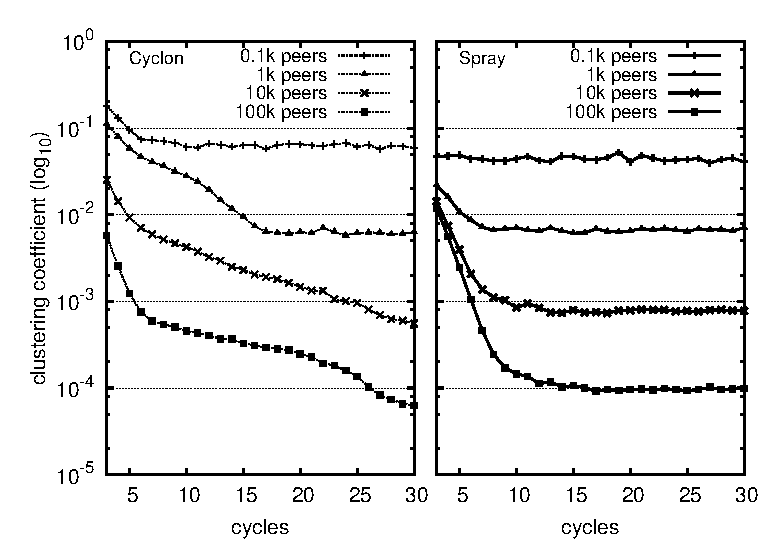
\includegraphics[width=0.49\textwidth]{img/simple.eps}
  \caption{\label{fig:clustering}Clustering coefficient.}
\end{figure}

\begin{asparadesc}
\item[Objective:] To observe how adaptiveness impacts clustering and convergence
  time.
\item[Description:] The average local clustering
  coefficient~\cite{watts1998collective} measures peers' neighborhood
  connectivity in the network:
  \begin{equation*}
    \overline{C} = {1\over |V^t|}\sum\limits_{x\in V^t}C_x
  \end{equation*}
  where $C_x$ is the local clustering coefficient of Peer $p_x$.  The
  runs concern 0.1k, 1k, 10k and 100k peers. The representative of the
  fixed-size approach is \CYCLON which is optimally configured for 1k
  peers: $\ln(1000)\approx 7$ neighbors. During exchanges, the peers
  using \CYCLON shuffle $3$ out of their $7$ neighbors. \CYCLON is
  oversized for 0.1k peers and undersized for 10k peers and 100k
  peers.
\item[Results:] Figure~\ref{fig:clustering} shows that \CYCLON starts
  with a lower clustering coefficient than \SPRAY. Still, \SPRAY
  converges faster than \CYCLON. Furthermore, when the number of peers
  in the network grows, the convergence time of \CYCLON suffers
  heavily. On the contrary, \SPRAY converges very quickly
  regardless of the network size. Figure~\ref{fig:clustering} also
  shows that both approaches converge to a low clustering coefficient
  which is characteristic of random graphs. Nevertheless, \CYCLON and
  \SPRAY do not reach the same values after convergence. Except when
  \CYCLON is optimally configured, \SPRAY's values are either below
  (when \CYCLON is oversized) or above (when \CYCLON is undersized).
  Overall, this shows that \SPRAY is
  \begin{inparaenum}
  \item faster to converge to a stable clustering coefficient
  \item reflecting the needs of the network membership.
  \end{inparaenum}
\item[Reasons:] \CYCLON starts with a lower clustering coefficient
  because each peer performs random walks to advertise themselves in
  the network. Hence, the starting overlay is already slightly
  balanced when the simulation starts the shufflings. On the other
  hand, a newcomer peer in \SPRAY only advertises itself to the
  neighborhood of its contact peer. Therefore, the network overlay
  starts strongly unbalanced, independently of the network
  size. Still, \CYCLON converges more slowly than \SPRAY because of
  its fixed-size partial view and the size of the shuffle. When they
  are configured \emph{a priori}, they constitute a constraint to the
  convergence speed.  The clustering coefficient measures how much the
  neighborhood of each peer is connected to the rest of the
  network. It directly depends on the partial view size of each peer
  which, in \CYCLON, is fixed. Thus, when the number of peers is
  multiplied by $10$, the clustering coefficient after convergence is
  divided by $10$. On the other hand, the peers using \SPRAY have
  variable-size partial views that reflect the network size with a
  logarithmic growth. Thus, when the network has 1k peers, the partial
  view size adapts to this network size. This explains the slightly
  larger view size of \SPRAY on this run (\SPRAY 7.4 vs \CYCLON 7). By
  extending the reasoning, this also explains why \SPRAY yields lower
  $\overline{C}$ values when \CYCLON is oversized, and why it yields
  higher values when \CYCLON is undersized.
\end{asparadesc}

\subsection{Information dissemination}

\begin{figure}
  \centering
  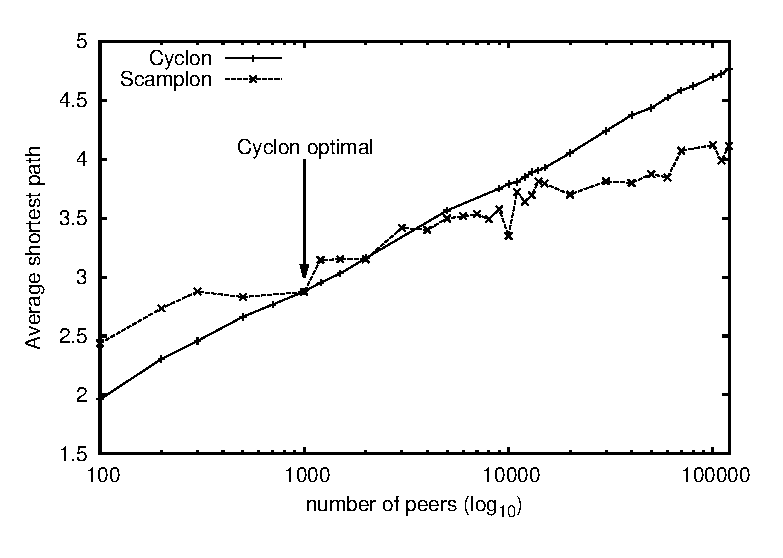
\includegraphics[width=0.49\textwidth]{img/avgpath.eps}
  \caption{\label{fig:avgpath}Average shortest path length.}
\end{figure}

\begin{asparadesc}
\item[Objective:] To observe how adaptiveness impacts the average shortest path
  length, i.e., the speed of information dissemination.
\item[Description:] The average path length is the average of the
  shortest path length between peers in the graph. It counts the
  minimum number of hops to reach a peer from another given peer. It
  basically represents the traveling time of any information to reach
  all the peers at least once. We average the path length on a subset
  of the network membership. We run the simulation on \SPRAY $100$
  times to avoid any side effects due to randomness. We also run the
  simulation on different configurations of \CYCLON targeting
  different optimal network sizes. \CYCLON with 7 neighbors targets 1k
  peers. \CYCLON with 9 neighbors targets 8k peers. \CYCLON with 11
  neighbors targets 60k peers. We perform the measurements after
  convergence. The checkpoints for the measurements are 0.1k, 0.5k,
  1k, 5k, 10k, 50k, and 100k peers.
\item[Results:] Figure~\ref{fig:avgpath} shows that both \CYCLON and
  \SPRAY have a relatively small average shortest path length. Thus,
  information reaches all peers very rapidly. Figure~\ref{fig:avgpath}
  also shows that each run of \CYCLON taken alone can be divided in
  three parts compared to \SPRAY. First, an oversized \CYCLON
  disseminates the information faster than \SPRAY. Then, \SPRAY and
  \CYCLON are equivalent where the latter is optimally
  configured. Finally, \SPRAY yields better results. Overall, \SPRAY
  scales better than \CYCLON since the gradient (slope) of the former is lower
  than any configuration of the latter.
\item[Reasons:] We perform all the measurements after convergence
  where the network overlay is closely related to random graphs. In
  such graph, the diameter and average shortest path length are small,
  hence the results of Figure~\ref{fig:avgpath}. The second
  observation concerns the comparison of each \CYCLON configuration
  with \SPRAY.  An oversized \CYCLON is much better connected into the
  graph and thus yields a lower average path length than
  \SPRAY. However, when \CYCLON is undersized, \SPRAY achieves better
  performance thanks to its larger partial views. Overall, \SPRAY
  scales better than any configuration of \CYCLON because it follows
  the optimal value for the size of partial views.
\end{asparadesc}


% \begin{figure*}
%   \centering
%   \subfloat[Figure A][\label{fig:churnA}Global number of arcs during an experiment 
%   including churn.]{
%     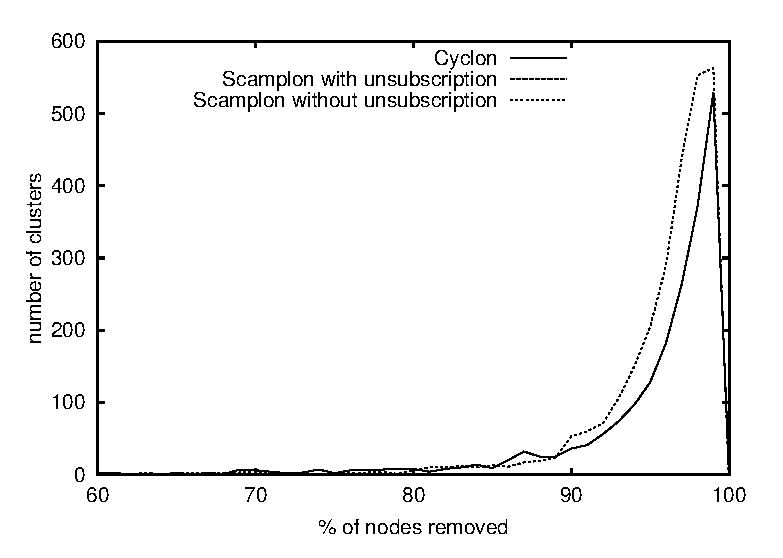
\includegraphics[width=0.48\textwidth]{img/churn.eps}}
%   \hspace{10pt}
%   \subfloat[Figure B][\label{fig:churnB}Average partial view size during an experiment
%   including churn.]{
%     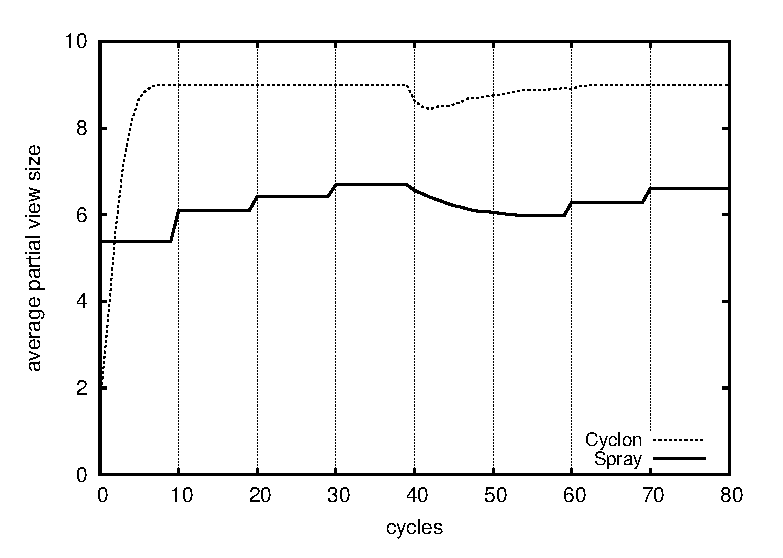
\includegraphics[width=0.48\textwidth]{img/avgpv.eps}}
% \end{figure*}

\subsection{Load-balancing}

\begin{figure}
  \centering
  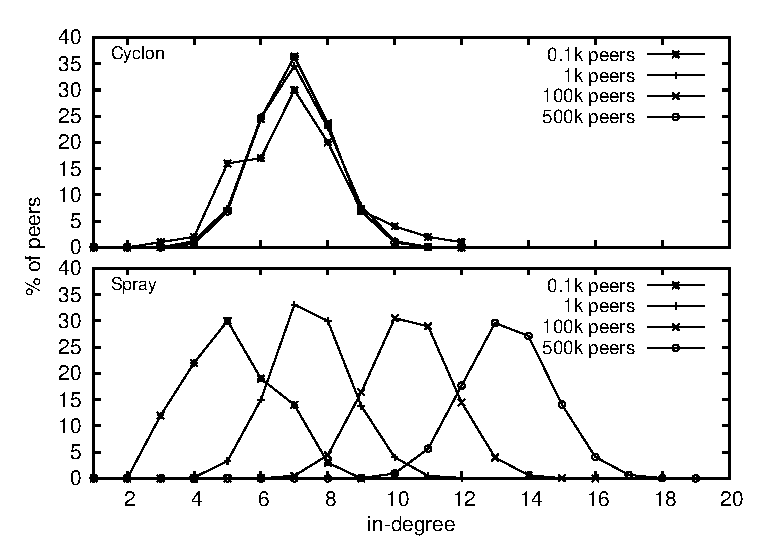
\includegraphics[width=0.49\textwidth]{img/histo.eps}
  \caption{\label{fig:histo}In-degree distribution.}
\end{figure}

\begin{asparadesc}
\item[Objective:] To observe how adaptiveness impacts the in-degree
  distribution, i.e., the load-balancing among peers.
\item[Description:] The in-degree of a peer shows how well it is
  represented in others' partial views. The in-degree distribution of
  the network highlights the existence of weakly connected peers and
  strongly connected hubs. This directly impacts robustness. In this
  experiment, the fixed-size partial view approach is \CYCLON{}. It is
  configured with partial views of size $7$ which targets a network 1k
  peers.  For all the experiments, we perform the in-degree
  measurements after convergence. The measurements concern networks
  with 0.1k, 1k, 100k, 500k peers.
\item[Results:] Figure~\ref{fig:histo} shows the in-degree
  distribution of \CYCLON and \SPRAY. In the top figure, we observe
  that the distribution and the degrees of \CYCLON are identical,
  independently of the network size. Thus, the distribution of 0.1k
  peers is identical to the 500k one with a mean value of roughly 7
  with a strong peak on this value. On the other hand, the bottom
  figure shows that the distribution of \SPRAY follows the average
  partial view size, which itself follows the growth of the size of
  the network. Figure~\ref{fig:histo} also shows that peers are very
  gathered around the mean partial view size. For instance, for the
  run with 500k peers using \SPRAY, the mean value for the in-degree
  is 13.37 and 88\% of the peers have an in-degree between 12 and 14
  included. This means that the load is well balanced among
  peers. Since peers are equally important in terms of connectedness,
  the network is robust to failures.
\item[Reasons:] Once configured, \CYCLON must handle any number of
  peers in the network with a fixed-size partial view and since the
  partial view size is constant, the in-degree of peers stays
  stable. 
  % Proportionally, the number of times
  % that a particular peer is referenced does not change compared to
  % the network
  % size. Indeed, the number of arcs that a new peer brings to the
  % network when it
  % joins constitutes that many arcs targeting it after the shuffling
  % rounds. S
  On the other hand, in \SPRAY, each joining peer brings an increasing
  number of arcs in the network. Thus, the in-degree of each peer
  grows reflecting the network size. Hence, the distribution in the
  bottom figure shifts slowly to higher in-degree values as the
  network size grows.  \SPRAY does not peak on a particular value as
  \CYCLON because the average partial view size for a particular
  network size falls in-between integer values. For instance, if the
  average partial view size is 6.5, then half of them have a size of 6
  while the other half have a size of 7. Such network is robust to
  failure because no peer is more important than others in term of
  connectedness. Therefore, if some random peer crashes, it will not
  affect the network as much as if a strongly connected peer crashed.
\end{asparadesc}

%%\vspace{-7pt}
%%\paragraph{Adaptive partial views}

\subsection{Adaptive partial view}

\begin{figure}
  \centering
  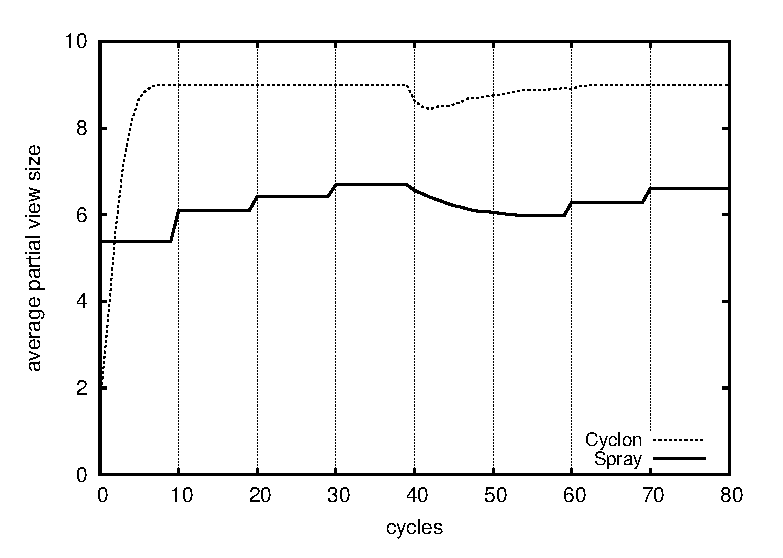
\includegraphics[width=0.49\textwidth]{img/avgpv.eps}
  \caption{\label{fig:churn}Average partial view size with churn.}
\end{figure}

\begin{asparadesc}

\item[Objective:] To show the impact of adaptiveness over partial view size when
  the network size grows and shrinks over time.
\item[Description:] In this experiment we focus on a dynamic network where peers
  can join and leave.  \CYCLON's configuration targets 8k peers. It is
  oversized compared the network size during the simulation (maximum 1k
  peers). During the first half of the experimentation, 250 peers are added 4
  times successively by intervals of 10 cycles each. Thus, the network size goes
  from 0 to 1k peers in 40 rounds. Then, half of the network leaves without
  giving notice (500 peers). Finally, 250 peers join two additional times. The
  final network contains 1k members. The measurements concern the average
  partial view size.
\item[Results:] Figure~\ref{fig:churn} shows the average partial view size of
  \SPRAY and \CYCLON. As expected, \CYCLON immediately converges to the
  configured partial view size (9 neighbors). On the other hand, \SPRAY's
  partial views logarithmically grow while the network grows. When the removals
  occur at cycle 40, the peers using \CYCLON remove the dead arcs while
  refilling their partial view until they reach the configured partial view
  size. \SPRAY only remove the arcs to reflect the departed peers. At the end,
  the \SPRAY partial views contain in average 6.6 neighbors (recall
  $\ln(1000)\approx 6.9$).
\item[Reasons:] Since each peer injects a logarithmically growing number of
  arcs, the average partial view size grows as more peers joins the network.
  The removal of 500 peers implies a decreasing slope. The slightly decreasing
  number of arcs after the removal is due to peers realizing that some arcs are
  dead, leading to a probabilistic removal (cf. Algorithm~\ref{algo:unreachable}).
\end{asparadesc}

% \vspace{-7pt}
% \paragraph{Robustness}

\subsection{Robustness}

\begin{figure}
  \centering
  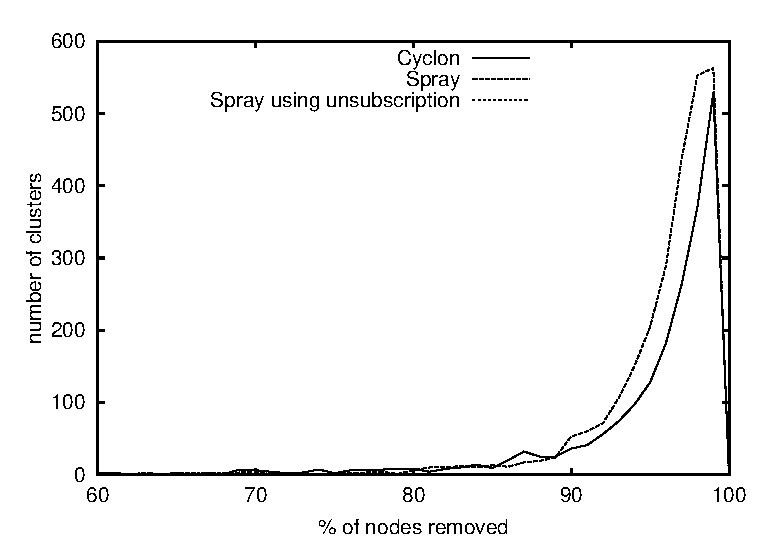
\includegraphics[width=0.49\textwidth]{img/resilience.eps}
  \caption{\label{fig:resilience}Robustness to massive failures.}
\end{figure}

\begin{asparadesc}
\item[Objective:] To show \SPRAY's robustness to failures.
\item[Description:] To evaluate robustness, we count the number of
  weakly and strongly connected components of the network. Counting
  strong components allows us to estimate the effectiveness of
  information dissemination protocols. For example, with two strong
  components, bidirectional communication between the two components
  cannot be achieved. But the network may still be in a repairable
  state.  For example, the first strong component may be able to reach
  the second, but the second may not reach the first. This happens if
  the two strong components constitute a single weak
  component. Counting the weak components therefore allows us to
  estimate to what extent the network can be repaired.  After some
  shuffling, a unidirectional link between two strong components may
  in fact give birth to one or more links in the other direction.

  In our experiment, we configure \CYCLON's view size to 9, which
  targets 8k peers. The network contains 10k members. We perform the
  removals after the approaches have converged to a stable overlay
  network. We remove a random set of peers at once, from 25 to 95 percent
  of peers every 5 percents, i.e., 16 runs for each approach. We
  perform a last measurement at 99 percent. We measure the number of
  components immediately after each removal.
\item[Results:] Figure~\ref{fig:resilience} shows the ratio of strong/weak
  components over the network size after removals. First, the figure shows that
  both the random peer sampling protocols \SPRAY and \CYCLON suffer from
  deteriorated behavior at high removal percentages, \CYCLON being slightly
  better in this term. Figure~\ref{fig:resilience} shows that the information
  dissemination (strong components) starts to slowly degrade at 45 percents, and
  quickly degrade at 70 percents. Fortunately, Figure~\ref{fig:resilience} also
  shows that the approaches are able to recover from such clustering until high
  removal rate. Indeed, the weak components start to increase at 70 percents,
  meaning that some part of the network are completely disjoint and beyond
  repair.%  Globally, Figure~\ref{fig:resilience} also demonstrates that the
  % logarithmic growth of these sampling protocols constitutes an upper bound, for
  % smaller growth could be obtained without endangering the connectedness of the
  % network.
\item[Reasons:] The random peer sampling approaches \CYCLON and \SPRAY
  yield very similar results because \CYCLON's configuration targets a
  network size of 8k peers, while \SPRAY adjusts itself automatically
  to this network size.  Therefore, the two protocols create very
  similar numbers of arcs. Yet \CYCLON performs slightly better for
  two reasons. First the variance in the degree distribution of \SPRAY
  causes \CYCLON to have more arcs in this specific
  experiment. Second, \SPRAY wastes some of its neighbors due to the
  presence of duplicate entries in its views (yet, the number of
  duplicates remains small cf. Figure~\ref{fig:duplicates}). Still
  both protocols preserve the ability to disseminate information until
  very large removal percentages. Another way to interpret this result
  consists in observing that when all peers have similar degrees,
  (cf. Figure~\ref{fig:histo}), removing a particular peer does not
  greatly affect connectedness. As suggested above, the direction of
  arcs impacts more information dissemination than the peer-sampling
  protocol itself. If an arc constitutes the last link between two
  clusters of the network, the messages from one of these clusters
  cannot reach the other one. Yet, this arc is enough for the
  peer-sampling protocol to start shuffling the views, ultimately
  populating them with members from both cluster. Hence, the network
  repairs itself.  When clusters become fully disjoints, neither
  \CYCLON nor \SPRAY is able to repair the
  network.  % A smaller growth could be obtained because the
  % sharp threshold of connectedness applies to random graphs according to Erd{\H
  %   o}s-R{\' e}nyi~\cite{erdos1959random}. However, random peer sampling
  % protocols constraint the partial views size to reduce the variance between
  % peers.  With such slight difference, we presume that a lower bound on arcs
  % growth could be found, although that may require global knowledge.
\end{asparadesc}

%%\vspace{-7pt}
%%\paragraph{Duplicates}

\subsection{Duplicates}

\begin{figure}
  \centering
  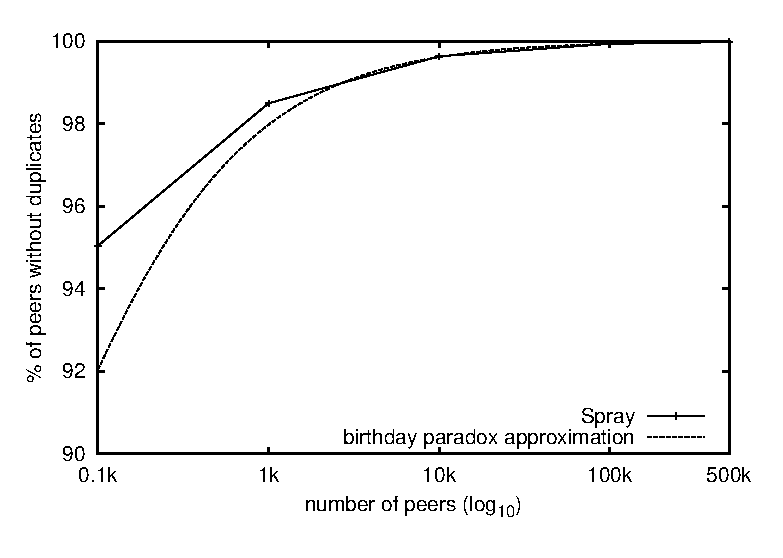
\includegraphics[width=0.49\textwidth]{img/duplicates.eps}
  \caption{\label{fig:duplicates}Duplicates in networks of different size.}
\end{figure}

\begin{asparadesc} 
\item[Objective:] To show that a small proportion of peers contains duplicates
  in their partial view.
\item[Description:] Using \SPRAY as random peer sampling protocol, we measure
  the amount of peers which have a partial view containing at least one
  duplicated reference. We perform the measurements on networks containing
  0.1k, 1k, 10k, 100k, and 500k peers. We measure the number of duplicates
  after convergence. We put this in relation with a theoretical approximation
  from the birthday paradox. The probability of a peer to not have duplicates
  is approximately:
  \begin{equation*}
    1- 
    (1-
    \exp({-\ln(|V^t|)*(\ln(|V^t|)-1)\over{2*|V^t|}}))
  \end{equation*}
\item[Results:] Figure~\ref{fig:duplicates} shows the proportion of peers using
  a partial view containing duplicates. We observe that there always exist
  partial views with at least one duplicate. The proportion is more important
  when the network size is small (e.g. 5 percents for 0.1k peers). It becomes a
  minor overhead when the network size is larger (e.g. less than 1 percent for
  10k peers). The birthday paradox approximation seems to follow very closely
  the experimental results. It empirically confirms that there exists a relation
  between the duplicates and the birthday paradox. The proportion of peers
  without duplicates tends to 100 percents as the network size grows.
\item[Reasons:] As the network grows, the chances of a particular peer to have
  at least twice the reference to another peer becomes smaller. Indeed, while
  the network grows linearly, the number of references to a particular peer
  only grows logarithmically. % Nevertheless, the birthday paradox reminds that
  % this proportion is not as small as it seems to be.
\end{asparadesc}


\subsection{Failures in connection establishment}
\label{subsec:degeneration}

\begin{figure}
  \centering 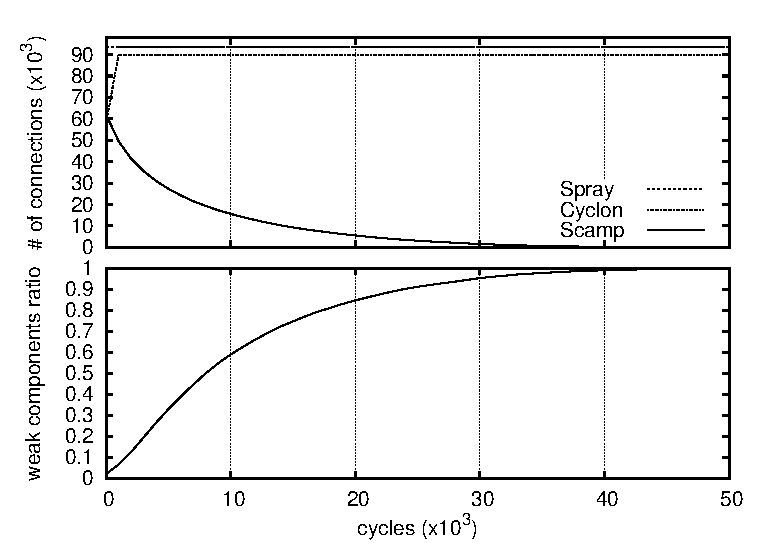
\includegraphics[width=0.49\textwidth]{img/degen.eps}
  \caption{\label{fig:degeneration}Number of arcs and partitioning in networks
    subject to failures in the connection establishments.}
\end{figure}

\begin{asparadesc}
\item[Objective:] To show that \SPRAY does not suffer from failures in
  connection establishments, contrarily to \SCAMP.
\item[Description:] We measure both the arc count and the number of weak
  components in the network. The simulations involve \CYCLON (configured with
  partial view containing 9 neighbors targeting a network of roughly 8k
  peers), \SCAMP\footnote{A modified version of \SCAMP whose periodic protocol
    works properly when there is no connection failures. Available at
    \url{https://github.com/justayak/peersim-spray}}, and \SPRAY. They run over
  50k cycles. The network initially contains 10k members.  To establish a
  connection, we use the WebRTC three-way handshake, i.e., the initial peer
  emits an offer ticket, the arrival peer stamps the ticket, the initial peer
  finalizes the connection using the stamped ticket
  (cf. Section~\ref{sec:relatedwork}). The probability that the ticket fails to
  traverse a hop is set to $10^{-3}$.
\item[Results:] Figure~\ref{fig:degeneration} has two parts. The top
  figure shows the arc count of the random peer samplings while the
  bottom figure shows the weak components of the network.  First, we
  observe that, as expected, the arc counts of \CYCLON and \SPRAY
  stays constant over cycles: 90k and 93k arcs for \CYCLON and \SPRAY
  respectively. Second, we observe that \SCAMP suffers from failures
  in connection establishment. This directly impacts network
  connectedness as measured by the weak-component ratio. The network
  of \SCAMP quickly degrades.
\item[Reasons:] The arc counts of \CYCLON and \SPRAY remains constant
  over time but for different reasons. In \CYCLON, the shuffling
  protocol makes sure that the partial view is filled to its
  maximum. When a peer removes a broken connection, it replaces it
  with a fresh one in the following round.  In \SPRAY, when the
  protocol tries to use a broken connection, it replaces it with
  another known one. Thus, the arc count stays constant and the
  shuffling protocol makes sure that duplicates disappear over time
  (the arc moves to another peer where it is not a duplicate).
  \SCAMP, however, does not establish new connections with the
  neighbors of its neighbors.  Each hop of connection establishment
  process is an opportunity for failure.  Let $P_f$ be the probability
  that an element of the dissemination path (either a peer or a
  connection) crashes or leaves during a hop of the three-way
  handshake, without any possible recovery. Let $P_E$ be the
  probability that a connection establishment cannot be
  completed. Without three-way handshake, $P_E$ is straightforward:
  \begin{equation} P_{E,\,1way}^{Scamp}=1-(1-
    P_f)^{k+1} \end{equation} This corresponds to the probability that
  each element (arc and peer) in the path of size $k+1$ stays alive
  during the random walk. In the context of WebRTC, the offer ticket
  must travel back to its emitter. As a consequence, the elements of
  the random walk cannot fail until the stamped ticket travels
  back. We obtain:
  \begin{align} P_{E,\,3way}^{Scamp} &=1 - ((1-P_f)^{2(k+1)} (1-P_f)^{2k}
                                       \ldots (1-P_f)^2) \nonumber \\
                                     &=1-(1-P_f)^{k^2+3k+2}
  \end{align}
  In other terms, the first chosen arc and peer in the path must stay
  alive $2k+2$ hops, the second chosen arc and peer must stay alive
  $2k$ hops and so on.  This long duration leads to a quicker
  degeneration of the connection count.

  % This behavior endangers the network
  % connectedness.%%, as depicted in Section~\ref{subsec:degeneration}.

  % Since there is no routing in such network, the only way for a stamped ticket
  % to come back to its emitter is the path it traveled in the first place. Hence,
  % all peers belonging to the path must stay alive until the stamped ticket comes
  % back in order to consistently forward it.  Furthermore, its periodic protocol
  % starts with an immediate cutting of the incoming arcs of the initiating peer
  % because it assumes that each connection spread in the network will establish.
  % Since it does not, the peer eventually becomes disconnected. Also, when its
  % neighbors execute the periodic protocol, they delete their reference in its
  % partial view. In such case, the peer becomes disconnected and partitions
  % quickly appear.
\end{asparadesc}

%%% Local Variables:
%%% mode: latex
%%% TeX-master: "../paper"
%%% End:
